\section{Exercice 5}
Nous souhaitons à présent envoyer des requêtes en traversant le proxy de l'ESIEE. Pour cela, nous réutilisons l'exercice 3 en passant des paramètres différents à la fonction \emph{create\_GET\_request()} de \emph{http\_tools.c}.\\

Le client doit tout d'abord se connecter au proxy de l'ESIEE et non plus directement au serveur web souhaité. Deux constantes \emph{ESIEE\_PROXY\_IP} et \emph{ESIEE\_PROXY\_PORT} ont ainsi été définies dans \emph{http\_tools.h} et sont ensuite utilisées pour se connecter (voir listing ci-dessous).

% FIXME coloration syntaxique
\begin{lstlisting}[caption=Extrait de http\_tools.h]
#define ESIEE_PROXY_IP "147.215.1.189"
#define ESIEE_PROXY_PORT "3128"
\end{lstlisting}
\

Pour qu'une requête HTTP puisse traverser un proxy, il faut que \emph{Request-URI} soit absolue. Nous devons donc passer l'URL complète du site web dans la requête. \emph{Host} quant-à-lui contient l'adresse du proxy.

\begin{lstlisting}[caption=Exemple de requête en passant par le proxy de l'ESIEE, language=bash]
GET http://www.google.com/ HTTP/1.1\r\n
Host: 147.215.1.189:3128\r\n
Connection: close\r\n
Accept: text/html\r\n\r\n
\end{lstlisting}
\

\noindent Ci-dessous un extrait du code de \emph{exo5/client.c} permettant d'effectuer les étapes décrites plus haut.

\begin{lstlisting}
    int sockfd, status;
    char *request;

    if (argc < 2) {
        printf(
            "Missing arguments\n"
            "Usage : %s full_URL\n"
            "Example: %s http://www.google.fr/\n",
            argv[0], argv[0]
        );
        return EXIT_FAILURE;
    }

    sockfd = init_stream_client_socket(ESIEE_PROXY_IP, atoi(ESIEE_PROXY_PORT));

    // Send request
    request = create_GET_request(ESIEE_PROXY_IP, argv[1], ESIEE_PROXY_PORT);
    if (request == NULL) {
        printf("client - could not create the GET request.");
        return EXIT_FAILURE;
    }

    ...
\end{lstlisting}
\newpage

\subsection{Exemple d'exécution}
\begin{figure}[h!]
	\centering
	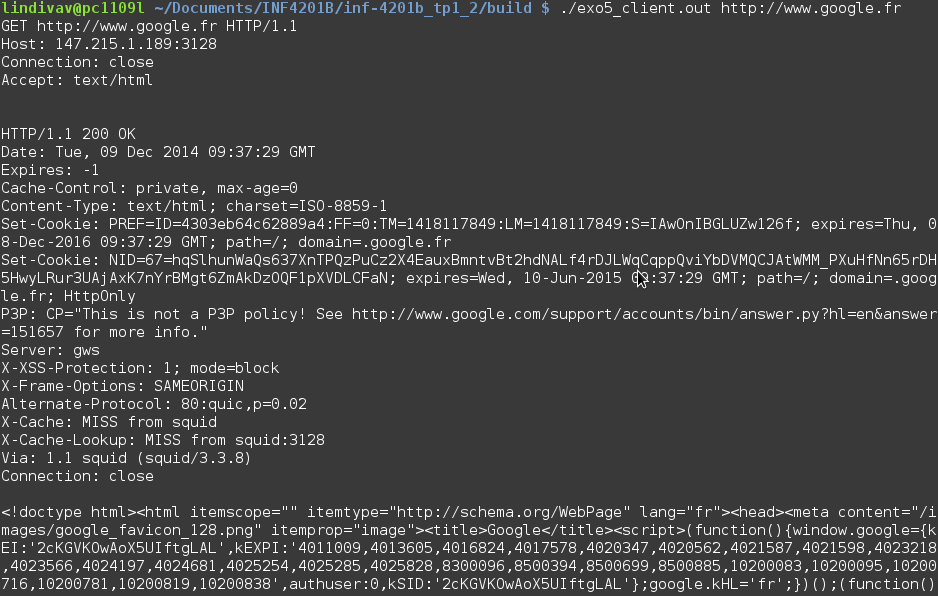
\includegraphics[width=1.0\textwidth]{screenshots/ex5.png}
	\caption{exo5\_client.out}
\end{figure}
